%% Machine Learning and Agentic AI for Macroeconomic Research
%% Lecture 4: Solving Macro Models via Deep Learning and Reinforcement Learning
%% Author: Zhigang Feng
%% Based on: 6-macro_model_ML/Lec_2026_6_ML_Macro.tex

\documentclass[10pt,english,aspectratio=169]{beamer}

\usepackage{ae,aecompl}
\usepackage[T1]{fontenc}
\usepackage{textcomp}
\usepackage[utf8]{inputenc}
\usepackage{babel}

\setcounter{secnumdepth}{3}
\setcounter{tocdepth}{3}

\usepackage{amsmath, amssymb, graphicx}
\usepackage{booktabs, multirow}
\usepackage{tikz}
\usetikzlibrary{positioning, calc, shapes.geometric, arrows.meta}
\usepackage{pgfplots}
\pgfplotsset{compat=1.18}
\usepackage{listings}
\usepackage{xcolor}

\lstset{
  basicstyle=\ttfamily\small,
  keywordstyle=\color{blue!80!black}\bfseries,
  commentstyle=\color{green!50!black}\itshape,
  stringstyle=\color{orange!80!black},
  backgroundcolor=\color{gray!8},
  frame=single,
  rulecolor=\color{gray!40},
  breaklines=true,
  showstringspaces=false,
  numbers=none,
}

\lstdefinestyle{pythonstyle}{
    language=Python,
    basicstyle=\ttfamily\footnotesize,
    keywordstyle=\color{blue!80!black}\bfseries,
    commentstyle=\color{green!50!black}\itshape,
    stringstyle=\color{orange!80!black},
    backgroundcolor=\color{gray!8},
    frame=single,
    rulecolor=\color{gray!40},
    breaklines=true,
    showstringspaces=false,
    numbers=left,
    numbersep=5pt,
    numberstyle=\tiny\color{gray}
}

\ifx\hypersetup\undefined
  \AtBeginDocument{%
    \hypersetup{bookmarks=false,breaklinks=true,pdfborder={0 0 0},colorlinks=true,
      linkcolor=DarkText,urlcolor=RedTitle}%
  }
\else
  \hypersetup{bookmarks=false,breaklinks=true,pdfborder={0 0 0},colorlinks=true,
    linkcolor=DarkText,urlcolor=RedTitle}%
\fi

\makeatletter
\newcommand\makebeamertitle{\frame{\maketitle}}%
\AtBeginDocument{%
  \let\origtableofcontents=\tableofcontents
  \def\tableofcontents{\@ifnextchar[{\origtableofcontents}{\gobbletableofcontents}}
  \def\gobbletableofcontents#1{\origtableofcontents}%
}

\usetheme{metropolis}
\usefonttheme{professionalfonts}

\definecolor{LightGray}{RGB}{230,230,230}
\definecolor{RedTitle}{RGB}{0,0,200}
\definecolor{VeryLightGray}{RGB}{245,245,245}
\definecolor{DarkText}{RGB}{0,0,0}

\setbeamercolor{background canvas}{bg=white}
\setbeamercolor{title}{fg=RedTitle}
\setbeamercolor{author}{fg=DarkText}
\setbeamercolor{date}{fg=DarkText}
\setbeamercolor{frametitle}{bg=VeryLightGray,fg=DarkText}
\setbeamercolor{normal text}{fg=DarkText}

\setbeamersize{text margin left=5mm, text margin right=5mm}
\addtobeamertemplate{frametitle}{}{\vspace{-0.5em}}
\newcommand{\reducevspace}{\vspace{-0.5cm}}

\setbeamertemplate{navigation symbols}{}
\setbeamertemplate{footline}{%
  \hfill%
  \usebeamercolor[fg]{page number in head/foot}%
  \usebeamerfont{page number in head/foot}%
  \insertframenumber\,/\,\inserttotalframenumber\kern1em\vskip2pt%
}

\makeatother

\graphicspath{{../../6-macro_model_ML/}}

\title[ML \& Agentic AI for Macro Research]{Machine Learning and Agentic AI for Macroeconomic Research\\
4: Solving Macro Models via Deep Learning \& RL\\[0.5em]}
\author{Zhigang Feng}
\date{Spring 2026}

\begin{document}

\makebeamertitle

%=============================================================================
% AGENDA
%=============================================================================

\begin{frame}{Lecture Agenda}
\begin{enumerate}
  \item \textbf{Motivation: Why Deep Learning for Macro Models?}
    --- the curse of dimensionality, function approximation, the ML opportunity
  \medskip
  \item \textbf{The Running Example: Optimal Growth Model}
    --- Bellman equation, VFI, analytical benchmark
  \medskip
  \item \textbf{Deep Learning Approach}
    --- parameterize value/policy functions with neural networks
  \medskip
  \item \textbf{Actor-Critic Algorithm for the Growth Model}
    --- two-network architecture, gradient-based updates
  \medskip
  \item \textbf{Euler Equation Method + Supervised Learning}
    --- Euler residual as loss function, training a policy network
  \medskip
  \item \textbf{Structured Neural Networks for Equilibrium}
    --- ICNN, monotonic networks, embedding economic theory
  \medskip
  \item \textbf{Accuracy, Validation, and Lab Preview}
    --- benchmarking against analytical solutions
\end{enumerate}
\end{frame}


%=============================================================================
% PART I: MOTIVATION
%=============================================================================
\section{Motivation: Why Deep Learning for Macro Models?}

%---------------------------------------
\begin{frame}{The Computational Frontier in Macro}
\begin{itemize}
  \item Quantitative macroeconomics solves dynamic optimization problems:
    \[
      V(k) = \max_{k'} \Big\{ u\big(f(k) - k'\big) + \beta\, V(k') \Big\}
    \]
  \item \textbf{Standard toolkit}: Value Function Iteration (VFI), Euler equation methods, perturbation
  \medskip
  \item These methods have served the profession well for decades
  \item But they face fundamental limitations as models grow richer:
    \begin{itemize}
      \item More state variables (capital, bonds, housing, human capital\ldots)
      \item Heterogeneous agents (wealth distributions, idiosyncratic risk)
      \item Aggregate uncertainty (business cycles in HA models)
    \end{itemize}
  \medskip
  \item \textbf{This lecture}: How deep learning and reinforcement learning offer a fundamentally different approach
\end{itemize}
\end{frame}

%---------------------------------------
\begin{frame}{The Naive Approach: Grid-Based Methods}
\begin{itemize}
  \item \textbf{Value Function Iteration on a grid}:
    \begin{enumerate}
      \item Discretize the state space: $\{k_1, k_2, \ldots, k_N\}$
      \item For each grid point, solve $\max_{k'} \{u(f(k_i) - k') + \beta V(k')\}$
      \item Iterate until convergence
    \end{enumerate}
  \medskip
  \item \textbf{This works well} when:
    \begin{itemize}
      \item The state space is low-dimensional (1--3 variables)
      \item The functions are smooth
      \item We can afford to evaluate $V$ at every grid point
    \end{itemize}
  \medskip
  \item Alternatives like Chebyshev polynomials and finite elements improve efficiency but share the same fundamental scaling problem
\end{itemize}
\end{frame}

%---------------------------------------
\begin{frame}{Why Grids Break: The Curse of Dimensionality}
\begin{itemize}
  \item With $N$ grid points per dimension and $d$ state variables:
    \[
      \text{Total grid points} = N^d
    \]
  \item \textbf{Example}: $N = 100$ points per dimension
    \begin{itemize}
      \item $d = 1$: $100$ points \quad (trivial)
      \item $d = 2$: $10{,}000$ points \quad (manageable)
      \item $d = 5$: $10^{10}$ points \quad (infeasible)
      \item $d = 10$: $10^{20}$ points \quad (absurd)
    \end{itemize}
  \medskip
  \item \textbf{Real macro models} often have $d \geq 5$:
    \begin{itemize}
      \item Krusell-Smith (1998): individual capital $k$ + aggregate capital $K$ + shocks
      \item Life-cycle models: age + assets + earnings + health + \ldots
      \item HA models with aggregate risk: the \emph{entire wealth distribution} is a state
    \end{itemize}
  \medskip
  \item Grid-based methods simply \textbf{cannot} scale to these problems
\end{itemize}
\end{frame}

%---------------------------------------
\begin{frame}{Beyond Grids: Other Classical Limitations}
\begin{itemize}
  \item \textbf{Perturbation methods} (linearization around steady state):
    \begin{itemize}
      \item Fast and accurate locally
      \item But may lose accuracy far from steady state
      \item Struggle with non-linearities, occasionally binding constraints, regime switches
    \end{itemize}
  \medskip
  \item \textbf{Projection methods} (Chebyshev, finite elements):
    \begin{itemize}
      \item Globally accurate for smooth problems
      \item Require structured grids or node sets
      \item Still suffer from the curse of dimensionality
    \end{itemize}
  \medskip
  \item \textbf{Kinks and non-convexities}:
    \begin{itemize}
      \item Borrowing constraints, irreversible investment, discrete choices
      \item First-order conditions fail or require complex root-finding
    \end{itemize}
  \medskip
  \item We need function approximators that scale gracefully with dimension and handle irregular structures
\end{itemize}
\end{frame}

%---------------------------------------
\begin{frame}{The Deep Learning Opportunity}
\begin{itemize}
  \item \textbf{Neural networks} are universal function approximators:
    \begin{itemize}
      \item Can represent any continuous function on a compact set (Cybenko 1989, Hornik et al.\ 1989)
      \item Parameter count grows \emph{polynomially} with dimension, not exponentially
    \end{itemize}
  \medskip
  \item \textbf{Automatic differentiation} provides gradients for free:
    \begin{itemize}
      \item No need to derive and code analytical derivatives
      \item Euler equations, FOCs, Jacobians --- all computed automatically
    \end{itemize}
  \medskip
  \item \textbf{GPU acceleration}:
    \begin{itemize}
      \item Matrix operations (forward/backward pass) are massively parallelizable
      \item Simulate thousands of economic agents simultaneously
    \end{itemize}
  \medskip
  \item \textbf{The key insight}: Recast the macro model as a \emph{learning problem} where the decision rule (policy) or value function is the object to be learned
\end{itemize}
\end{frame}

%---------------------------------------
\begin{frame}{The Inspiration: AlphaGo and Economic Models}
\begin{itemize}
  \item \textbf{AlphaGo} (DeepMind, 2016) solved a problem with $\sim 10^{170}$ possible board states
  \item It did \emph{not} enumerate the state space or solve the full Bellman equation on a grid
  \medskip
  \item \textbf{It used two neural networks}:
    \begin{itemize}
      \item \textbf{Policy Net (Actor)}: ``Intuition'' --- which move to play
      \item \textbf{Value Net (Critic)}: ``Judgment'' --- who is winning
    \end{itemize}
  \medskip
  \item \textbf{Lesson for economics}: When the state space is too vast to enumerate (like the wealth distribution in a HA model), we can use the same two-network approach
  \medskip
  \item \textbf{This lecture}: Apply this actor-critic idea to the optimal growth model as a proof of concept, then discuss how it scales to richer models
\end{itemize}
\end{frame}

%---------------------------------------
\begin{frame}{Reframing Macro as a Machine Learning Problem}
\begin{itemize}
  \item The optimal growth model can be recast as a \textbf{learning problem}:
    \begin{itemize}
      \item The decision rule $g(k)$ is approximated by a neural network
      \item The first-order conditions provide a natural \textbf{loss function}
      \item Modern optimization (Adam, SGD) and automatic differentiation drive training
    \end{itemize}
  \medskip
  \item \textbf{Two complementary approaches}:
    \begin{enumerate}
      \item \textbf{Deep Value Function Iteration}: Train networks to satisfy the Bellman equation (reinforcement learning flavor)
      \item \textbf{Euler Equation Minimization}: Train a network to satisfy the FOCs (supervised learning flavor)
    \end{enumerate}
  \medskip
  \item Both use the same building blocks:
    \begin{itemize}
      \item Neural network function approximation
      \item Stochastic gradient descent
      \item Monte Carlo sampling of state space
    \end{itemize}
\end{itemize}
\end{frame}


%=============================================================================
% PART II: THE RUNNING EXAMPLE
%=============================================================================
\section{Running Example: The Optimal Growth Model}

%---------------------------------------
\begin{frame}{Optimal Growth Model: Setup}
\begin{itemize}
  \item \textbf{Objective}: Maximize discounted lifetime utility:
    \[
      \max_{\{k_{t+1}\}} \sum_{t=0}^{\infty} \beta^t u\Big(f(k_t) - k_{t+1}\Big)
    \]
  \item \textbf{Production function}: $f(k_t) = k_t^\alpha$
  \item \textbf{Resource constraint}: Consumption $c_t = f(k_t) - k_{t+1}$
  \item \textbf{Depreciation}: $\delta = 1$ (full depreciation) in our benchmark; adjustable for general cases
  \medskip
  \item \textbf{Steady-state capital}:
    \[
      k_{ss} = \left(\frac{1}{\alpha\beta}\right)^{\frac{1}{\alpha - 1}} = (\alpha\beta)^{\frac{1}{1-\alpha}}
    \]
  \medskip
  \item \textbf{Why this model?} Simple enough for an analytical solution (ground truth), yet contains all the essential structure of richer models
\end{itemize}
\end{frame}

%---------------------------------------
\begin{frame}{Bellman Equation and VFI}
\begin{itemize}
  \item \textbf{Recursive formulation} (Bellman equation):
    \[
      V(k) = \max_{k'} \Big\{ u\big(f(k) - k'\big) + \beta\, V(k') \Big\}
    \]
  \item \textbf{Value Function Iteration}:
    \begin{enumerate}
      \item Start with initial guess $V^0(k)$
      \item Update: $V^{n+1}(k) = \max_{k'}\{u(f(k) - k') + \beta\, V^n(k')\}$
      \item Repeat until $\|V^{n+1} - V^n\| < \text{tolerance}$
    \end{enumerate}
  \medskip
  \item \textbf{Contraction Mapping Theorem}: Under standard assumptions, the Bellman operator $T$ is a contraction with modulus $\beta$
    \begin{itemize}
      \item Guarantees convergence to unique fixed point $V^*$
      \item This is the theoretical foundation we build on
    \end{itemize}
\end{itemize}
\end{frame}

%---------------------------------------
\begin{frame}{Stochastic Extension}
\begin{itemize}
  \item Add a productivity shock $z$:
    \[
      v(y) = \max_{0 \leq c \leq y} \Big\{ u(c) + \beta\, \mathbb{E}\big[v(y')\big] \Big\}
    \]
  \item Transition: $y' = f(y - c)\cdot z$, where $z$ is i.i.d.\ log-normal
  \medskip
  \item \textbf{Analytical solution} for log utility $u(c) = \ln(c)$ and Cobb-Douglas $f(k) = k^\alpha$:
    \begin{align*}
      V^*(y) &= A + B \ln y \quad \text{(value function)} \\
      c^*(y) &= (1 - \alpha\beta)\, y \quad \text{(optimal policy: consume fixed fraction)}
    \end{align*}
  \medskip
  \item This closed-form solution serves as our \textbf{ground truth} for validating all neural network methods
  \item Lab 6A builds this benchmark via classical VFI with interpolation
\end{itemize}
\end{frame}

%---------------------------------------
\begin{frame}{VFI with Interpolation: The Classical Algorithm}
\begin{itemize}
  \item Since $y$ is continuous, we use interpolation on a grid:
  \medskip
  \begin{enumerate}
    \item \textbf{Initialize}: Grid $\{y_1, \ldots, y_N\}$, initial guess $v^0$
    \item \textbf{Interpolate}: Create function $\hat{v}(y)$ connecting $(y_i, v^0_i)$ pairs
    \item \textbf{Bellman update}: For each $y_i$:
      \[
        v^{\text{new}}_i = \max_c \left\{\ln(c) + \beta \sum_j \hat{v}\big(f(y_i - c)\, z_j\big)\, \phi(z_j)\right\}
      \]
    \item \textbf{Check convergence}: If $\|v^{\text{new}} - v^0\| < \text{tol}$, stop; else repeat
  \end{enumerate}
  \medskip
  \item This is the \textbf{benchmark} algorithm implemented in Lab 6A
  \item Works beautifully for 1D\ldots but the grid makes it impractical for higher dimensions
\end{itemize}
\end{frame}


%=============================================================================
% PART III: DEEP LEARNING APPROACH
%=============================================================================
\section{Deep Learning Approach: NNs for Value and Policy Functions}

%---------------------------------------
\begin{frame}{The Core Idea: Replace Grids with Neural Networks}
\begin{itemize}
  \item \textbf{Instead of} storing $V(k)$ on a grid, \textbf{approximate} it with a neural network:
    \[
      V(k) \approx \Gamma_{\gamma_v}(k), \qquad g(k) \approx \Gamma_{\gamma_g}(k)
    \]
    where $\gamma_v, \gamma_g$ are network parameters (weights and biases)
  \medskip
  \item \textbf{The analogy to VFI}:
    \begin{enumerate}
      \item Generate states $k \sim d(k)$ from some distribution (replaces grid)
      \item Compute approximate target values or gradients for training
      \item Update $\gamma_v$ or $\gamma_g$ using gradient-based optimization
    \end{enumerate}
  \medskip
  \item \textbf{Why this helps}: Neural networks handle high-dimensional $k$ naturally
    \begin{itemize}
      \item No grid needed --- states are \emph{sampled}
      \item The network generalizes across the state space
      \item Parameters grow polynomially, not exponentially, with dimension
    \end{itemize}
\end{itemize}
\end{frame}

%---------------------------------------
\begin{frame}{Embedding Equilibrium Conditions in Neural Networks}
\begin{itemize}
  \item Neural network approximations can incorporate \textbf{equilibrium conditions} directly:
    \begin{itemize}
      \item \textbf{Feasibility constraints}: Ensure $g(k) \in \mathcal{G}(k)$
        \begin{itemize}
          \item Example: $0 \leq c \leq f(k)$ (can't consume more than output)
        \end{itemize}
      \item \textbf{Market clearing}: $\sum_i c_i = Y$ or asset market clearing
      \item \textbf{Budget constraints}: Household or government budget balance
    \end{itemize}
  \medskip
  \item \textbf{Implementation strategies}:
    \begin{enumerate}
      \item \textbf{Output transformations}: Sigmoid $\to$ bound outputs within feasible range
      \item \textbf{Penalty methods}: Add constraint violation terms to the loss
      \item \textbf{Lagrangian approaches}: Dual variables updated during training
      \item \textbf{Architectural design}: Structure the network so outputs automatically satisfy identities
    \end{enumerate}
  \medskip
  \item Building in economic structure improves convergence and ensures economically meaningful solutions
\end{itemize}
\end{frame}

%---------------------------------------
\begin{frame}{Value Function Update (One-Step Look-Ahead)}
\begin{itemize}
  \item Fix a policy $g^{(n-1)}(k) = \Gamma_{\gamma_g}^{(n-1)}(k)$
  \item The one-step approximation for the value is:
    \[
      \hat{V}(k) = u\bigl(k, g^{(n-1)}(k)\bigr) + \beta\, \Gamma_{\gamma_v}^{(n-1)}\bigl(f(k, g^{(n-1)}(k))\bigr)
    \]
  \item We then solve a \textbf{least squares} problem:
    \[
      \min_{\gamma_v^{(n)}} \; \frac{1}{N_v}\sum_{i=1}^{N_v} \Bigl(\Gamma_{\gamma_v}^{(n)}(k_i) - \hat{V}(k_i)\Bigr)^2
    \]
  \medskip
  \item \textbf{Key}: States $\{k_i\}$ are \emph{sampled} from distribution $d(k)$, not placed on a grid
  \item This is \textbf{supervised learning}: the ``label'' for each $k_i$ is the Bellman target $\hat{V}(k_i)$
\end{itemize}
\end{frame}

%---------------------------------------
\begin{frame}{The Role of Value Function in Policy Evaluation}
\begin{itemize}
  \item Note that $\Gamma_{\gamma_v}^{(n-1)}(k)$ is \textbf{fixed} when computing $\hat{V}(k)$
  \medskip
  \item \textbf{Key insight}: The value network serves as an \emph{evaluator} of the current policy:
    \begin{itemize}
      \item If $\Gamma_{\gamma_v}^{(n-1)} \approx V^*$ and $g^{(n-1)} \approx g^*$, then $\hat{V}(k) \approx V^*(k)$
    \end{itemize}
  \medskip
  \item \textbf{On the expectation operator}: $\mathbb{E}_{k \sim d(k)}[\cdot]$ averages over the \emph{state space}, not over stochastic uncertainty
    \begin{itemize}
      \item Even in deterministic models, we average over sampled states
      \item \textbf{Rationale}: If a candidate policy performs well \emph{on average} across all sampled states, it must be a good approximation globally
      \item Poor average performance signals the policy is inadequate somewhere
    \end{itemize}
  \medskip
  \item This ``average fitness'' criterion ensures robust approximation across the entire domain
\end{itemize}
\end{frame}

%---------------------------------------
\begin{frame}{Policy Function Update}
\begin{itemize}
  \item Given the updated value network $\Gamma_{\gamma_v}^{(n)}$, improve the policy by solving:
    \[
      \max_{\gamma_g^{(n)}} \;\; \frac{1}{N_g}\sum_{i=1}^{N_g}\Bigl[ u\bigl(k_i, \Gamma_{\gamma_g}^{(n)}(k_i)\bigr) + \beta\, \Gamma_{\gamma_v}^{(n)}\bigl(f(k_i, \Gamma_{\gamma_g}^{(n)}(k_i))\bigr) \Bigr]
    \]
  \item This is \textbf{gradient ascent} on the neural network parameters:
    \[
      \gamma_g^{(n)} = \gamma_g^{(n-1)} + \alpha \cdot \nabla_{\gamma_g} J(\gamma_g)\Big|_{\gamma_g = \gamma_g^{(n-1)}}
    \]
  \medskip
  \item \textbf{Two roles of the gradient}:
    \begin{enumerate}
      \item \textbf{Direction}: $\nabla_{\gamma_g} J$ tells us \emph{which direction} in parameter space improves the objective
      \item \textbf{Magnitude}: Combined with learning rate $\alpha$, determines \emph{how far} we move
    \end{enumerate}
  \medskip
  \item In practice, optimizers like Adam adaptively adjust step sizes for faster and more stable convergence
\end{itemize}
\end{frame}

%---------------------------------------
\begin{frame}{Choosing the Sampling Distribution $d(k)$}
\begin{itemize}
  \item The distribution $d(k)$ determines \emph{where} we evaluate the approximation
  \medskip
  \item \textbf{Common choices}:
    \begin{itemize}
      \item \textbf{Uniform}: Simple, but wastes capacity on unlikely states
      \item \textbf{Stationary distribution}: Focuses on states the economy actually visits
      \item \textbf{Importance sampling}: Targets high-uncertainty or high-value regions
    \end{itemize}
  \medskip
  \item \textbf{Stationary distribution approach}:
    \begin{enumerate}
      \item Simulate the economy under current policy for many periods
      \item Wait until the state converges to its ergodic distribution
      \item Draw training points from that distribution
    \end{enumerate}
  \medskip
  \item \textbf{Benefits}: Sample efficiency (focus on what matters), faster convergence, no need for a handcrafted grid
  \item \textbf{Limitation}: Rare but important events (tail risks) may be under-represented
\end{itemize}
\end{frame}


%---------------------------------------
\begin{frame}{Why Not Chebyshev Here?}
\begin{itemize}
  \item Chebyshev and finite-element methods must approximate over the \emph{entire} domain
  \item As dimensionality grows, covering the entire domain becomes infeasible
  \medskip
  \item \textbf{Stationarity-based sampling} zooms in on the \emph{likely} region of interest
  \medskip
  \item \textbf{Possible concerns and remedies}:
    \begin{itemize}
      \item \textbf{Rare but important events}: Combine stationary sampling with targeted sampling of rare states (importance sampling)
      \item \textbf{Multiple steady states}: A single stationary distribution might miss transient states
      \item \textbf{Out-of-distribution robustness}: Conduct stress tests separately
    \end{itemize}
  \medskip
  \item The combination of \textbf{Monte Carlo sampling} (generates the right data in relevant states) and \textbf{neural networks} (fits irregular, mesh-free data) is the key synergy
\end{itemize}
\end{frame}

%---------------------------------------
\begin{frame}{Bias-Variance Tradeoff: One-Step vs.\ Multi-Step}
\begin{itemize}
  \item \textbf{One-step} ($T_{\text{sim}} = 1$):
    \[
      \hat{V}(k_i) = u\bigl(k_i, g(k_i)\bigr) + \beta\, \Gamma_{\gamma_v}(k_{i,1})
    \]
    \begin{itemize}
      \item[$+$] Easy to implement, low variance
      \item[$-$] High bias if $V(\cdot)$ approximation is poor
    \end{itemize}
  \medskip
  \item \textbf{$T_{\text{sim}}$-step return}:
    \[
      \hat{V}(k_i) = \sum_{t=0}^{T_{\text{sim}}-1} \beta^t\, u(k_{i,t}, g(k_{i,t})) + \beta^{T_{\text{sim}}}\, \Gamma_{\gamma_v}(k_{i,T_{\text{sim}}})
    \]
    \begin{itemize}
      \item[$+$] Lower bias: uses actual simulated rewards over multiple steps
      \item[$-$] Higher variance: simulated paths can vary significantly
    \end{itemize}
  \medskip
  \item \textbf{In practice}: Choose $T_{\text{sim}}$ to balance bias vs.\ variance; Lab 6B uses $T_{\text{sim}} = 30$--$50$
\end{itemize}
\end{frame}


%=============================================================================
% PART IV: ACTOR-CRITIC ALGORITHM
%=============================================================================
\section{Actor-Critic Algorithm for the Growth Model}
% Note: We develop the full RL theory (Monte Carlo, TD, actor-critic)
% in Lecture 5. Here we apply the actor-critic idea to the growth model.

%---------------------------------------
\begin{frame}{Why Actor-Critic? The Optimization Bottleneck}
\emph{Preview: we develop the full RL theory in Lecture~5; here we apply the actor-critic idea to the growth model.}
\medskip
\begin{itemize}
  \item \textbf{Classical VFI} requires solving $\max_{k'} Q(k, k')$ at every state
  \item When $Q$ is represented by a neural network (non-convex), this inner maximization is expensive and unreliable
  \medskip
  \item \textbf{The actor-critic solution}: Use \emph{two} networks to avoid the inner max:
    \begin{enumerate}
      \item \textbf{The Actor (Policy Net $\pi$)} --- ``The Doer''
        \begin{itemize}
          \item Input: state $k$ $\to$ Output: action $k'$ directly
          \item \emph{Avoids} the expensive maximization step
        \end{itemize}
      \item \textbf{The Critic (Value Net $V$)} --- ``The Judge''
        \begin{itemize}
          \item Input: state $k$ $\to$ Output: estimated value $V(k)$
          \item Minimizes the \textbf{Bellman residual} (prediction error)
        \end{itemize}
    \end{enumerate}
  \medskip
  \item The actor proposes actions; the critic evaluates them; both improve iteratively
\end{itemize}
\end{frame}

%---------------------------------------
\begin{frame}{Mapping Macroeconomics to Reinforcement Learning}
\vspace{-0.3cm}
To apply RL, we translate economic models into the standard tuple $(S, A, P, R, \gamma)$:

\vspace{0.2cm}
\begin{table}[]
\centering
\renewcommand{\arraystretch}{1.4}
\scriptsize
\begin{tabular}{l | l | l}
\textbf{RL Concept} & \textbf{Economic Equivalent} & \textbf{Note} \\
\hline
\textbf{Agent} & Household / Firm & The optimizer \\
\hline
\textbf{Environment} & Constraints \& Prices & The rules of the game \\
\hline
\textbf{State ($S$)} & $(k, z, \Delta)$ & Wealth, shocks, \textbf{distribution} \\
\hline
\textbf{Action ($A$)} & $c, i, l$ & Consumption, investment \\
\hline
\textbf{Transition ($P$)} & $k' = (1-\delta)k + i$ & \textbf{Micro}: Known perfectly \\
& $\Delta' = H(\Delta)$ & \textbf{Macro}: Often unknown/intractable \\
\hline
\textbf{Reward ($R$)} & $u(c)$ & Period utility \\
\hline
\textbf{Discount ($\gamma$)} & $\beta$ & Time preference \\
\end{tabular}
\end{table}

\vspace{0.2cm}
\textbf{The synergy}: RL handles the complexity of the macro transition $\Delta' = H(\Delta)$ by simply \emph{simulating} it, without needing to derive the law of motion explicitly
\end{frame}

%---------------------------------------
\begin{frame}{The Actor-Critic Algorithm: Overview}
\begin{enumerate}
  \item \textbf{Initialize}: Policy network $\Gamma_{\gamma_g}^{(0)}$, Value network $\Gamma_{\gamma_v}^{(0)}$
  \medskip
  \item \textbf{Policy Evaluation} (update the Critic):
    \begin{itemize}
      \item Generate training data $\{k_i, \hat{V}(k_i)\}$ using $T_{\text{sim}}$-step Monte Carlo simulation
      \item Solve: $\min_{\gamma_v^{(n)}} \sum_i [\Gamma_{\gamma_v}^{(n)}(k_i) - \hat{V}(k_i)]^2$
    \end{itemize}
  \medskip
  \item \textbf{Policy Improvement} (update the Actor):
    \begin{itemize}
      \item Generate states $\{k_i\}$ (e.g., from stationary distribution)
      \item Solve: $\max_{\gamma_g^{(n)}} \sum_i [u(k_i, \Gamma_{\gamma_g}^{(n)}(k_i)) + \beta\, \Gamma_{\gamma_v}^{(n)}(f(k_i, \Gamma_{\gamma_g}^{(n)}(k_i)))]$
    \end{itemize}
  \medskip
  \item \textbf{Check convergence} and repeat until $\Gamma_{\gamma_g}$ and $\Gamma_{\gamma_v}$ stabilize
\end{enumerate}
\end{frame}

%---------------------------------------
\begin{frame}{Addressing the Infinite Horizon}
\textbf{The puzzle}: Macro models maximize over an infinite horizon ($\sum_{t=0}^\infty \beta^t u_t$), but Monte Carlo simulations are always finite.

\vspace{0.3cm}
\textbf{The solution: Bootstrapping}
\begin{itemize}
  \item We don't need to simulate to infinity
  \item We use the \textbf{estimated value function} (Critic) as a proxy for the infinite future:
    \[
      \text{Total Value} \approx \underbrace{\sum_{t=0}^{T-1} \beta^t u_t}_{\text{Simulated rewards}} + \beta^T \underbrace{\hat{V}(s_T)}_{\text{Learned proxy for } \sum_{t=T}^\infty}
    \]
  \medskip
  \item This allows learning infinite-horizon policies using only short simulation rollouts
  \item The Critic improves over time, making the bootstrap estimate more accurate
\end{itemize}
\end{frame}

%---------------------------------------
\begin{frame}{Monte Carlo and Uncertainty}
\begin{itemize}
  \item When the model includes \textbf{stochastic shocks}, the future state evolves randomly
  \item Enumerating all possible future states or integrating over a high-dimensional shock space quickly becomes infeasible (another curse of dimensionality)
  \medskip
  \item \textbf{Monte Carlo simulation} circumvents this:
    \begin{itemize}
      \item Generate a large sample of realized state-and-shock paths
      \item Compute empirical averages to approximate expectations
      \item No need to explicitly deal with the full distribution
    \end{itemize}
  \medskip
  \item \textbf{In practice}:
    \begin{itemize}
      \item Choose $T_{\text{sim}}$ to balance bias vs.\ variance
      \item Use parallel or GPU-based Monte Carlo for large simulation demands
      \item Combine with importance sampling if rare shocks are of interest
    \end{itemize}
\end{itemize}
\end{frame}

%---------------------------------------
\begin{frame}{Advantage I: Flexible Function Approximation}
\begin{itemize}
  \item \textbf{Old way --- Structured grids}:
    \begin{itemize}
      \item Requires tensor product grids or sparse grids (Smolyak)
      \item Adding one state variable \emph{multiplies} the grid size
    \end{itemize}
  \medskip
  \item \textbf{New way --- Neural networks}:
    \begin{itemize}
      \item Universal approximators: can represent any continuous function
      \item Parameter count grows linearly/polynomially with dimension, \emph{not} exponentially
      \item Can handle high-dimensional states (entire shock histories, fine-grained distributions) that break grid-based methods
    \end{itemize}
  \medskip
  \item \textbf{Result}: Models that were previously intractable become solvable
\end{itemize}
\end{frame}

%---------------------------------------
\begin{frame}{Advantage II: The ``Mesh-Free'' Synergy}
Why is the combination of \textbf{Monte Carlo} and \textbf{deep learning} so powerful?

\begin{itemize}
  \item \textbf{Monte Carlo simulation} produces a ``cloud'' of points concentrated in the \textbf{ergodic set} (economically relevant states)
    \begin{itemize}
      \item Traditional interpolators (Chebyshev, splines) \emph{fail} on such irregular, clustered data (Runge's phenomenon)
    \end{itemize}
  \medskip
  \item \textbf{Neural networks are ``mesh-free''}:
    \begin{itemize}
      \item They do not require a grid
      \item They simply minimize error on \emph{whatever} points you give them
    \end{itemize}
  \medskip
  \item \textbf{Conclusion}: MC generates the \emph{right data} (relevant states), and DL is the \emph{right tool} to fit that irregular data
\end{itemize}
\end{frame}

%---------------------------------------
\begin{frame}{Advantage III: Hardware Acceleration}
\begin{itemize}
  \item \textbf{Parallelism}:
    \begin{itemize}
      \item Simulate thousands of economic agents in parallel on a GPU
      \item Neural network training (matrix multiplication) is highly optimized for GPUs/TPUs
    \end{itemize}
  \medskip
  \item \textbf{Comparison}:
    \begin{itemize}
      \item Traditional VFI is often serial or hard to parallelize efficiently
      \item Deep RL scales up naturally: more agents, more shocks $\to$ just add more compute
    \end{itemize}
  \medskip
  \item \textbf{Practical implication}: Models that took hours or days can now be solved in minutes
    \begin{itemize}
      \item Enables rapid iteration on model specification
      \item Makes calibration and estimation feasible for complex models
    \end{itemize}
\end{itemize}
\end{frame}


%=============================================================================
% PART V: EULER EQUATION METHOD
%=============================================================================
\section{Euler Equation Method + Supervised Learning}

%---------------------------------------
\begin{frame}{Context: Two Approaches to the Same Problem}
\begin{itemize}
  \item We have seen the \textbf{actor-critic} approach: train two networks to satisfy the Bellman equation
  \medskip
  \item Now we consider an alternative: \textbf{Euler equation minimization}
    \begin{itemize}
      \item Derive the first-order conditions (Euler equations)
      \item Train a \emph{single} policy network to satisfy them
    \end{itemize}
  \medskip
  \item \textbf{Comparison}:
    \begin{itemize}
      \item Actor-Critic (Bellman): Two networks, no need to derive FOCs, RL flavor
      \item Euler Equation: One network, requires deriving FOCs, supervised learning flavor
    \end{itemize}
  \medskip
  \item Both are valid; which is better depends on the model:
    \begin{itemize}
      \item Euler equation method is very precise when FOCs are available
      \item Actor-Critic is more general (handles kinks, discrete choices)
    \end{itemize}
\end{itemize}
\end{frame}

%---------------------------------------
\begin{frame}{The Euler Equation: Optimality Condition}
\begin{itemize}
  \item Capital accumulation: $k' = g(k)$, \quad consumption: $c = f(k) + (1-\delta)k - g(k)$
  \medskip
  \item For CRRA utility $u(c) = \frac{c^{1-\sigma}}{1-\sigma}$ and Cobb-Douglas production, the equilibrium satisfies:
    \[
      u'(c) = \beta\, u'(c')\, \bigl[\alpha\, g(k)^{\alpha-1} + 1 - \delta\bigr]
      \tag{EE}
    \]
  \medskip
  \item \textbf{Interpretation}: The marginal cost of saving today equals the discounted marginal benefit tomorrow
  \medskip
  \item \textbf{Goal}: Learn a policy $g$ that makes the \textbf{Euler residual} vanish:
    \[
      \mathcal{R}(k; g) = u'(c) - \beta\, u'(c')\bigl[\alpha\, g(k)^{\alpha-1} + 1 - \delta\bigr]
    \]
    for all economically relevant $k$
\end{itemize}
\end{frame}

%---------------------------------------
\begin{frame}{Euler Equation: Necessary but Not Sufficient}
\begin{itemize}
  \item \textbf{Important caveat}: The Euler equation is a \emph{necessary} condition for optimality, but \textbf{not sufficient} by itself
  \medskip
  \item For a complete characterization, we also need:
    \begin{itemize}
      \item \textbf{Transversality condition}: $\lim_{t\to\infty} \beta^t u'(c_t)\, k_{t+1} = 0$
      \item \textbf{Feasibility constraints}: $c \geq 0$, $k' \geq 0$
    \end{itemize}
  \medskip
  \item \textbf{Handling inequality constraints}:
    \begin{itemize}
      \item Kuhn-Tucker complementary slackness conditions arise
      \item Can be converted to equalities via Fischer-Burmeister functions or penalty methods
      \item Or handled via architectural constraints (sigmoid output)
    \end{itemize}
  \medskip
  \item For now, we focus on \textbf{interior solutions} where the Euler equation holds with equality throughout
\end{itemize}
\end{frame}

%---------------------------------------
\begin{frame}{From Euler Residual to Loss Function}
\begin{itemize}
  \item Approximate the policy by a neural network: $g(k) \approx \Gamma_{\gamma_g}(k)$
  \medskip
  \item Sample $k_i \sim d(k)$ (e.g., stationary distribution or uniform)
  \medskip
  \item Define the \textbf{mean-squared Euler residual} loss:
    \[
      \mathcal{L}_g(\gamma_g) = \frac{1}{N}\sum_{i=1}^{N} \bigl[\mathcal{R}(k_i; \Gamma_{\gamma_g})\bigr]^2
    \]
  \medskip
  \item \textbf{This is supervised learning}: the ``label'' for each state $k_i$ is zero (the Euler equation should hold exactly)
  \medskip
  \item Optimal policy parameters satisfy: $\nabla_{\gamma_g}\, \mathcal{L}_g(\gamma_g^*) = 0$
  \item All derivatives computed automatically via \texttt{autograd}
\end{itemize}
\end{frame}

%---------------------------------------
\begin{frame}{The Mean Value Intuition}
\begin{itemize}
  \item We minimize the \emph{average} Euler residual across sampled states:
    \[
      \mathcal{L}_g(\gamma_g) = \mathbb{E}_{k \sim d(k)}\bigl[\mathcal{R}(k; \Gamma_{\gamma_g})^2\bigr] \approx \frac{1}{N}\sum_{i=1}^{N} \mathcal{R}(k_i; \Gamma_{\gamma_g})^2
    \]
  \medskip
  \item \textbf{Intuition}:
    \begin{itemize}
      \item If a candidate policy satisfies the Euler equation \emph{on average} across all sampled states, it should be a good approximation to the true equilibrium policy
      \item If the average residual is large, the policy must be violating optimality somewhere
    \end{itemize}
  \medskip
  \item This ``average fitness'' criterion:
    \begin{itemize}
      \item Ensures global accuracy across the domain
      \item Is computationally tractable via Monte Carlo sampling
      \item Naturally integrates with gradient-based NN training
    \end{itemize}
\end{itemize}
\end{frame}

%---------------------------------------
\begin{frame}{Neural Network for the Policy Function}
\begin{itemize}
  \item Two-hidden-layer MLP (64--64--1) with ReLU and Sigmoid:
\end{itemize}
\[
  \boxed{
    \Gamma_{\gamma_g}(k) = \sigma_2\Bigl(W_2 \cdot \sigma_1(W_1 k + b_1) + b_2\Bigr)
  }
\]
\begin{itemize}
  \item Hidden activation $\sigma_1$ = \texttt{ReLU}; output activation $\sigma_2$ = \texttt{Sigmoid}
  \item Sigmoid output is scaled to $[0, f(k) + (1-\delta)k - \varepsilon]$ to ensure feasibility:
    \[
      0 \leq \Gamma_{\gamma_g}(k) \leq f(k) + (1-\delta)k
    \]
  \medskip
  \item All derivatives $\partial \mathcal{L}_g / \partial \gamma_g$ are computed automatically by \texttt{autograd}
  \item No need to derive or code analytical Jacobians
\end{itemize}
\end{frame}

%---------------------------------------
\begin{frame}{Minimising the Euler Residual: Training Loop}
\begin{itemize}
  \item Initialize $\gamma_g^{(0)}$; choose learning rate $\alpha_g$
  \medskip
  \item \textbf{Repeat until convergence}:
    \begin{enumerate}
      \item Draw a mini-batch $\{k_i\}_{i=1}^{B}$
      \item Compute loss $\mathcal{L}_g(\gamma_g)$ and its gradient via back-propagation
      \item Gradient step:
        \[
          \gamma_g^{(j+1)} = \gamma_g^{(j)} - \alpha_g\, \nabla_{\gamma_g} \mathcal{L}_g(\gamma_g^{(j)})
        \]
      \item Optionally resample $k_i$ from the same distribution $d(k)$
    \end{enumerate}
  \medskip
  \item \textbf{Pros of Euler method}:
    \begin{itemize}
      \item Very precise policy functions; theoretically grounded
      \item Only one network to train (simpler than actor-critic)
    \end{itemize}
  \item \textbf{Cons}: Does not yield the value function $V$; requires deriving FOCs
\end{itemize}
\end{frame}


%=============================================================================
% PART VI: PYTORCH IMPLEMENTATION
%=============================================================================
\section{PyTorch Implementation}

%---------------------------------------
\begin{frame}{Implementation Overview: Two Approaches}
\begin{itemize}
  \item We implement both approaches in PyTorch:
  \medskip
  \item \textbf{Approach 1 --- Euler Equation (Lab 6B, Part 1)}:
    \begin{itemize}
      \item Single \texttt{PolicyNetwork} with constrained output
      \item Loss: Mean squared Euler error
      \item Result: Policy function $g(k)$
    \end{itemize}
  \medskip
  \item \textbf{Approach 2 --- Deep Value Function Iteration (Lab 6B, Part 2)}:
    \begin{itemize}
      \item Two networks: \texttt{PolicyNet} + \texttt{ValueNet}
      \item $T$-step lookahead with soft constraints
      \item Result: Both policy $g(k)$ and value function $V(k)$
    \end{itemize}
  \medskip
  \item Both validated against the analytical solution from Lab 6A
\end{itemize}
\end{frame}

%---------------------------------------
\begin{frame}[fragile]{Network Architecture: PolicyNet and ValueNet}
\vspace{-0.3cm}
\begin{lstlisting}[style=pythonstyle,basicstyle=\ttfamily\tiny]
class ValueNet(nn.Module):
    def __init__(self, nh=64):
        super().__init__()
        self.net = nn.Sequential(
            nn.Linear(1, nh), nn.ReLU(),
            nn.Linear(nh, nh), nn.ReLU(),
            nn.Linear(nh, 1))
    def forward(self, k): return self.net(k)

class PolicyNet(nn.Module):
    def __init__(self, alpha, eps, nh=64):
        super().__init__()
        self.alpha, self.eps = alpha, eps
        self.net = nn.Sequential(
            nn.Linear(1, nh), nn.ReLU(),
            nn.Linear(nh, nh), nn.ReLU(),
            nn.Linear(nh, 1), nn.Sigmoid())  # Output in [0, 1]
    def forward(self, k):
        max_kp = torch.clamp(k**self.alpha - self.eps, 1e-9)
        return self.net(k) * max_kp  # Scale to [0, f(k)-eps]
\end{lstlisting}
\vspace{-0.3cm}
\begin{itemize}
  \item \texttt{Sigmoid} ensures $g(k) \in [0, f(k) - \varepsilon]$: feasibility by construction
  \item \texttt{ValueNet}: unconstrained output (value can be any real number)
\end{itemize}
\end{frame}

%---------------------------------------
\begin{frame}[fragile]{Policy Evaluation: Bellman MSE}
\vspace{-0.3cm}
\begin{lstlisting}[style=pythonstyle,basicstyle=\ttfamily\tiny]
def value_update_step(self):
    self.value_optimizer.zero_grad()
    # Sample batch of capital states
    k_batch = torch.rand(self.n_batch, 1, device=self.device) \
              * (self.k_max - self.k_min) + self.k_min

    v_current = self.value_net(k_batch)           # V(k)
    kp_batch  = self.policy_net(k_batch)           # k' = g(k)
    u_batch   = self.utility(k_batch, kp_batch)    # u(c)
    v_next    = self.value_net(kp_batch).detach()   # V(k') -- detach!
    bellman_rhs = u_batch + self.beta * v_next      # u + beta*V(k')

    loss = nn.functional.mse_loss(v_current, bellman_rhs)
    loss.backward()
    self.value_optimizer.step()
    return loss.item()
\end{lstlisting}
\vspace{-0.3cm}
\begin{itemize}
  \item Minimizes $\mathbb{E}[(V(k) - (u + \beta V(k')))^2]$
  \item \texttt{detach()}: prevents gradients from flowing through $V(k')$ --- treats the target as fixed
\end{itemize}
\end{frame}

%---------------------------------------
\begin{frame}[fragile]{Policy Improvement: Gradient Ascent}
\vspace{-0.3cm}
\begin{lstlisting}[style=pythonstyle,basicstyle=\ttfamily\tiny]
def policy_step(self):
    self.policy_optimizer.zero_grad()
    # Sample batch of capital states
    k_batch = torch.rand(self.n_batch, 1, device=self.device) \
              * (self.k_max - self.k_min) + self.k_min

    kp_batch = self.policy_net(k_batch)              # k' = g(k)
    u_batch  = self.utility(k_batch, kp_batch)       # u(c)
    v_next   = self.value_net(kp_batch)               # V(k')

    objective = torch.mean(u_batch + self.beta * v_next)

    loss = -objective   # Maximize objective = Minimize -objective
    loss.backward()
    self.policy_optimizer.step()
    return objective.item()
\end{lstlisting}
\vspace{-0.3cm}
\begin{itemize}
  \item Maximizes $\mathbb{E}[u(k, g(k)) + \beta\, V(g(k))]$
  \item Gradients flow through \textbf{both} $u$ and $V$ into the policy network parameters
\end{itemize}
\end{frame}

%---------------------------------------
\begin{frame}[fragile]{The Training Loop: Alternating Updates}
\vspace{-0.3cm}
\begin{lstlisting}[style=pythonstyle,basicstyle=\ttfamily\tiny]
def train(self):
    print(f"Training started on device={self.device}")
    pbar = tqdm(range(self.n_epoch), desc="Outer Loop")

    for _ in pbar:
        # Phase 1: Update Value Net (several inner steps)
        for _ in range(self.n_inner_value):
            v_loss = self.value_update_step()
        self.value_losses.append(v_loss)

        # Phase 2: Update Policy Net (several inner steps)
        for _ in range(self.n_inner_policy):
            policy_obj = self.policy_update_step()
        self.policy_objectives.append(policy_obj)

        pbar.set_postfix({
            "ValueLoss": f"{v_loss:.4e}",
            "PolicyObj": f"{policy_obj:.4e}"
        })
\end{lstlisting}
\vspace{-0.3cm}
\begin{itemize}
  \item Alternates between updating the Critic and the Actor
  \item Multiple inner steps per outer iteration for stability
\end{itemize}
\end{frame}

%---------------------------------------
\begin{frame}{Deep Value Function Iteration (DVFI): Key Innovations}
Lab 6B, Part 2 introduces three innovations beyond the basic actor-critic:

\begin{enumerate}
  \item \textbf{Unified Objective ($J$)}: $T$-step discounted sum plus terminal value:
    \[
      J(y_0) = \sum_{t=0}^{T-1} \beta^t u(c_t) + \beta^T V(y_T)
    \]
  \medskip
  \item \textbf{$T$-Step Lookahead}: Simulate the economy for $T = 30$--$50$ periods
    \begin{itemize}
      \item Gradients ``see'' long-term consequences of policy choices
      \item Reduces bias compared to one-step bootstrapping
    \end{itemize}
  \medskip
  \item \textbf{Soft Constraints} (penalty method):
    \begin{itemize}
      \item If $c > 0$: $u = \ln(c)$ \quad (standard)
      \item If $c \leq 0$: $u = \text{Penalty} \times (c - \varepsilon)$ \quad (pushes back to feasibility)
      \item Avoids hard clamping that kills gradients
    \end{itemize}
\end{enumerate}
\end{frame}

%---------------------------------------
\begin{frame}{DVFI: Separated Training Phases}
\begin{itemize}
  \item \textbf{Phase A --- Policy Net} (maximize $J$):
    \begin{itemize}
      \item Sample initial states $y_0$ uniformly in $[y_{\min}, y_{\max}]$
      \item Simulate $T$ periods using PolicyNet
      \item Compute $J = \sum \beta^t u(c_t) + \beta^T V(y_T)$
      \item Minimize $-J$ (gradient ascent on expected reward)
    \end{itemize}
  \medskip
  \item \textbf{Phase B --- Value Net} (fit $V$ to $J$):
    \begin{itemize}
      \item Target: $J$ from Phase A, \textbf{detached} from policy gradients
      \item Loss: $\|V(y_0) - J\|^2$ (standard regression)
    \end{itemize}
  \medskip
  \item \textbf{Key detail}: \texttt{retain\_graph=True} allows both phases to share the same computation graph; \texttt{detach()} in Phase B prevents policy updates through the value loss
\end{itemize}
\end{frame}


%=============================================================================
% PART VII: STRUCTURED NEURAL NETWORKS
%=============================================================================
\section{Structured Neural Networks for Equilibrium Models}

%---------------------------------------
\begin{frame}{The Computational Challenge in Quantitative Macro}
\begin{itemize}
  \item \textbf{Nested ``Russian Doll'' structure}: Quantitative macro models involve \emph{multiple} nested optimization problems
  \medskip
  \item \textbf{Typical hierarchy}:
    \begin{enumerate}
      \item \textbf{Outer Loop}: Market clearing / calibration (solve for prices $p^*$)
      \item \textbf{Middle Loop}: Value function iteration (solve Bellman equations)
      \item \textbf{Inner Loop}: Agent optimization (choose $c, \ell, k'$ given state and prices)
    \end{enumerate}
  \medskip
  \item \textbf{Problem with unstructured nets}: Approximating value functions or costs with generic FFNNs turns the \emph{inner} problem into a non-convex optimization
    \begin{itemize}
      \item Multiple local optima and unstable outer iterations
      \item Economic misspecification (e.g., upward-sloping demand, non-concave value functions)
    \end{itemize}
\end{itemize}
\end{frame}

%---------------------------------------
\begin{frame}{Idea: Inject Economic Structure into the Network}
\textbf{Key idea}: Design architectures that \emph{respect} economic shape restrictions \emph{by construction}.

\vspace{0.3cm}
\centering
\begin{table}[]
\renewcommand{\arraystretch}{1.4}
\begin{tabular}{l | l | l}
\textbf{Property} & \textbf{Mathematical Gain} & \textbf{Economic Payoff} \\
\hline
\textbf{Convexity / Concavity} & Unique global optimum & Stable policy rules / VFI \\
\hline
\textbf{Monotonicity} & Invertible mappings & Well-behaved supply/demand \\
\hline
\textbf{Homogeneity} & $f(\lambda x) = \lambda f(x)$ & Consistency with balanced growth \\
\end{tabular}
\end{table}

\vspace{0.3cm}
\begin{itemize}
  \item This turns the neural net from a \textbf{black box} into a \textbf{glass box}: flexible enough to fit data, but disciplined by theory
\end{itemize}
\end{frame}

%---------------------------------------
\begin{frame}{Baseline: Standard Feed-Forward Networks}
\textbf{Generic FFNN architecture}:
\begin{itemize}
  \item Composition of affine maps and nonlinearities:
    \[
      y = f_\theta(x) = W_L\, \sigma\bigl(\ldots \sigma(W_1 x + b_1)\bigr)
    \]
  \item Layer weights $W^{(l)} \in \mathbb{R}^{d_l \times d_{l-1}}$ are \textbf{unconstrained}
\end{itemize}

\vspace{0.2cm}
\textbf{The optimization trap}:
\begin{itemize}
  \item Even if the \emph{true} value function is concave, the FFNN approximation generally is not
  \item When agents optimize against this approximation:
    \begin{itemize}
      \item FOCs are necessary but not sufficient
      \item Numerical solvers can converge to spurious local optima
      \item Comparative statics and equilibrium mappings can be erratic
    \end{itemize}
  \medskip
  \item \textbf{Solution}: Constrain the network architecture to guarantee the desired shape
\end{itemize}
\end{frame}

%---------------------------------------
\begin{frame}{Input Convex Neural Networks (ICNN)}
\framesubtitle{Amos, Xu \& Kolter (ICML 2017)}
\textbf{Goal}: Construct $f(x)$ that is convex in $x$ \emph{by design}.

\vspace{0.2cm}
\textbf{Recursive definition}:
\[
  z_{l+1} = \sigma_l\left(\sum_{i=0}^l W_{l,i}^{(z)} z_i + W_l^{(x)} x + b_l\right)
\]

\textbf{Sufficient conditions for convexity}:
\begin{enumerate}
  \item \textbf{Non-negative recurrent weights}: all $W_{l,i}^{(z)} \geq 0$
  \item \textbf{Convex, non-decreasing activations}: $\sigma_l$ is convex and non-decreasing (e.g., ReLU, Softplus)
\end{enumerate}

\textbf{Result}:
\begin{itemize}
  \item $f(x)$ is convex in $x$ as a composition of convex, non-decreasing functions
  \item \textbf{Crucially}: Direct input weights $W_l^{(x)}$ can be \textbf{unconstrained} (including negative)
  \item This allows the network to learn the linear placement and slope freely
\end{itemize}
\end{frame}

%---------------------------------------
\begin{frame}{Why Impose Convexity in Macro?}
\small
Using ICNNs for value functions $V$ or pricing kernels delivers three benefits:

\begin{enumerate}
  \item \textbf{Robust Value Function Iteration}
    \begin{itemize}
      \item We solve $\max_{x'}\{u(x,x') + \beta\, \hat{V}(x')\}$
      \item If $\hat{V}$ is concave (or $-\hat{V}$ convex via ICNN), the objective is globally concave
      \item Fast, gradient-based \emph{convex} optimization with no local-maxima issues
    \end{itemize}

  \item \textbf{Well-Behaved Equilibrium Prices}
    \begin{itemize}
      \item Convex preferences $\Rightarrow$ monotone demand
      \item Unique, stable market-clearing price vectors
    \end{itemize}

  \item \textbf{Scalability to High Dimensions}
    \begin{itemize}
      \item ICNNs scale to high-dimensional state spaces while retaining the structure needed for Bellman contractions
    \end{itemize}
\end{enumerate}
\end{frame}

%---------------------------------------
\begin{frame}{ICNN: Proof Sketch (Why It's Convex)}
We prove by induction that each $z_l(x)$ is convex in $x$.

\vspace{0.2cm}
\textbf{Step 1: Base Case}
\begin{itemize}
  \item $z_0(x) = x$ is linear, hence convex \checkmark
\end{itemize}

\vspace{0.2cm}
\textbf{Step 2: Inductive Step}
\[
  z_{l+1}(x) = \sigma\bigl(W_z^{(l)} z_l(x) + W_x^{(l)} x + b_l\bigr)
\]
\begin{itemize}
  \item By induction, $z_l(x)$ is convex
  \item With $W_z^{(l)} \geq 0$: $W_z^{(l)} z_l(x)$ is a non-negative sum of convex functions $\Rightarrow$ convex
  \item Adding linear term $W_x^{(l)} x + b_l$ preserves convexity
  \item Applying convex, non-decreasing $\sigma(\cdot)$ to a convex argument preserves convexity \checkmark
\end{itemize}

\vspace{0.15cm}
\textbf{Therefore}: All layers $z_l(x)$, and hence $f(x)$, are convex in $x$
\end{frame}


%---------------------------------------
\begin{frame}{Do Constraints Limit Expressivity?}
\textbf{The concern}: By restricting $W_z \geq 0$, do we lose the universal approximation property?

\vspace{0.3cm}
\textbf{Theorem} (Chen, Man \& Amos, 2019):
\begin{quote}
An Input Convex Neural Network can approximate \emph{any} convex function over a compact domain to arbitrary accuracy.
\end{quote}

\vspace{0.2cm}
\textbf{Intuition}:
\begin{itemize}
  \item A maximum of affine functions ($\max_i\{a_i^\top x + b_i\}$) is convex and can approximate any convex shape
  \item An ICNN with ReLU activations acts as a hierarchical max-affine approximator
\end{itemize}

\textbf{Implication for macro}:
\begin{itemize}
  \item You are not imposing a specific parametric form (like CES or Cobb-Douglas)
  \item You are imposing a \textbf{shape restriction} (convexity) while retaining non-parametric flexibility
\end{itemize}
\end{frame}

%---------------------------------------
\begin{frame}{Partial Convexity: The Macro Reality}
\textbf{The issue}: Value functions $V(k, z)$ are typically:
\begin{itemize}
  \item \textbf{Concave} in endogenous states $k$ (capital, assets)
  \item \textbf{Non-concave / arbitrary} in exogenous states $z$ (TFP, income shocks)
\end{itemize}
A standard ICNN would incorrectly enforce convexity on $z$ as well.

\vspace{0.3cm}
\textbf{The solution: Partial ICNN (PICNN)}

Modify the architecture to distinguish between convex inputs ($u$) and non-convex inputs ($v$):
\[
  z_{l+1} = \sigma\left(\underbrace{W_z^{(l)} z_l}_{\geq 0} + \underbrace{W_u^{(l)}(u \circ v)}_{\text{interaction}} + \underbrace{W_v^{(l)} v}_{\text{free}} + b_l\right)
\]

\textbf{Implementation}: Pass $k$ through the ``convex path'' (constrained weights); pass $z$ through a standard FFNN path; combine such that convexity w.r.t.\ $k$ is preserved
\end{frame}

%---------------------------------------
\begin{frame}{Optimization Landscapes: FFNN vs.\ ICNN}
\begin{columns}
  \begin{column}{0.4\textwidth}
    \textbf{Standard FFNN}
    \begin{itemize}
      \item Rugged, non-convex landscape
      \item Many local minima
      \item Outcome depends on initialization
    \end{itemize}

    \vspace{0.3cm}

    \textbf{ICNN}
    \begin{itemize}
      \item Smooth, convex basin
      \item Unique global minimum
      \item Optimization is predictable
    \end{itemize}
  \end{column}

  \begin{column}{0.6\textwidth}
    \centering
    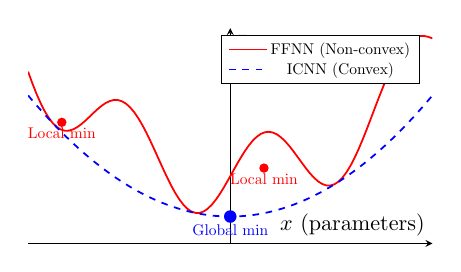
\begin{tikzpicture}[scale=0.8]
      \begin{axis}[
        width=8cm, height=5cm,
        axis lines=center,
        xlabel=$x$ (parameters), ylabel=Loss,
        xtick=\empty, ytick=\empty,
        ymin=0, ymax=8, xmin=-3, xmax=3,
        legend pos=north east,
        legend style={nodes={scale=0.7, transform shape}}
      ]
        \addplot[red, thick, domain=-3:3, samples=100]
          {0.5*x^2 + 1.5*sin(deg(3*x)) + 2.5};
        \addlegendentry{FFNN (Non-convex)}

        \addplot[blue, thick, dashed, domain=-3:3, samples=100]
          {0.5*x^2 + 1};
        \addlegendentry{ICNN (Convex)}

        \node[circle,fill=red,inner sep=1.5pt] at (axis cs:-2.5, 4.5) {};
        \node[red, below, scale=0.7] at (axis cs:-2.5, 4.5) {Local min};
        \node[circle,fill=red,inner sep=1.5pt] at (axis cs:0.5, 2.8) {};
        \node[red, below, scale=0.7] at (axis cs:0.5, 2.8) {Local min};

        \node[circle,fill=blue,inner sep=2pt] at (axis cs:0, 1) {};
        \node[blue, below, scale=0.7] at (axis cs:0, 0.9) {Global min};
      \end{axis}
    \end{tikzpicture}
  \end{column}
\end{columns}
\end{frame}

%---------------------------------------
\begin{frame}[fragile]{ICNN: Robust PyTorch Implementation}
\textbf{Strategy}: Use reparameterization (Softplus) instead of clamping to enforce $W_z \geq 0$.
\vspace{-0.2cm}
\begin{lstlisting}[style=pythonstyle,basicstyle=\ttfamily\tiny]
class ICNN(nn.Module):
    def __init__(self, d_in, hidden_sizes):
        super().__init__()
        # Passthrough weights (Input -> Hidden) [unconstrained]
        self.W_x = nn.ParameterList([
            nn.Parameter(torch.randn(h, d_in))
            for h in hidden_sizes])
        # Recurrent weights (Hidden -> Hidden) [unconstrained params]
        # Apply Softplus() during forward pass to enforce W_z >= 0
        self.W_z_params = nn.ParameterList([
            nn.Parameter(torch.randn(h, h_prev))
            for h, h_prev in zip(hidden_sizes[1:], hidden_sizes[:-1])])
        self.biases = nn.ParameterList([
            nn.Parameter(torch.zeros(h)) for h in hidden_sizes])

    def forward(self, x):
        z = x
        for i, (Wz_p, Wx, b) in enumerate(
                zip(self.W_z_params, self.W_x, self.biases)):
            Wz = F.softplus(Wz_p)  # Enforce non-negativity
            z_next = F.linear(z, Wz) + F.linear(x, Wx) + b
            z = F.relu(z_next)
        return z
\end{lstlisting}
\end{frame}

%---------------------------------------
\begin{frame}{Monotonic Neural Networks}
\begin{columns}
  \begin{column}{0.5\textwidth}
    \textbf{Objective}: Ensure $f(x)$ is non-decreasing:
    \[
      x_i \uparrow \;\Rightarrow\; f(x) \uparrow
    \]

    \vspace{0.2cm}
    \textbf{Two necessary constraints}:
    \begin{enumerate}
      \item \textbf{Non-negative weights}: $W^{(l)} \geq 0$ for all layers (biases unconstrained)
      \item \textbf{Monotonic activations}: $\sigma'(\cdot) \geq 0$ (ReLU, Sigmoid, Tanh, Softplus)
    \end{enumerate}

    \vspace{0.2cm}
    \textbf{Enforcement}: Same two methods as ICNN
    \begin{itemize}
      \item Clamping: simple but can kill neurons
      \item Reparameterization (Softplus): preferred
    \end{itemize}
  \end{column}

  \begin{column}{0.5\textwidth}
    \centering
    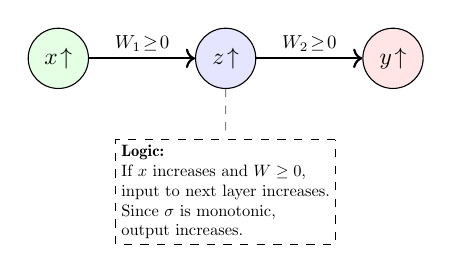
\begin{tikzpicture}[scale=0.85, transform shape,
      neuron/.style={circle, draw, minimum size=0.9cm},
      arrow/.style={->, thick}
    ]
      \node[neuron, fill=green!10] (I) at (0,0) {$x\!\uparrow$};
      \node[neuron, fill=blue!10] (H) at (2.5,0) {$z\!\uparrow$};
      \node[neuron, fill=red!10] (O) at (5,0) {$y\!\uparrow$};

      \draw[arrow] (I) -- (H) node[midway, above, scale=0.8] {$W_1 \!\geq\! 0$};
      \draw[arrow] (H) -- (O) node[midway, above, scale=0.8] {$W_2 \!\geq\! 0$};

      \node[draw, dashed, align=left, scale=0.7] at (2.5, -2) {
        \textbf{Logic:} \\
        If $x$ increases and $W \geq 0$, \\
        input to next layer increases.\\
        Since $\sigma$ is monotonic, \\
        output increases.
      };
      \draw[dashed, gray] (H) -- (2.5, -1.1);
    \end{tikzpicture}
  \end{column}
\end{columns}
\end{frame}

%---------------------------------------
\begin{frame}{Worked Example: Recovering Preferences via ICNN}
\textbf{Economic problem: Expenditure minimization}
\begin{align*}
  E(p, u) &= \min_{c \geq 0}\; p \cdot c \\
  \text{s.t.}\quad & U_\theta(c) \geq u \quad \text{(target utility)}
\end{align*}

\textbf{The ``structured'' solution}:
\begin{itemize}
  \item Learn the expenditure function $E_\theta(p, u)$ using a Concave ICNN
  \item \textbf{Theory}: $E(p, u)$ must be concave in prices $p$ (Shephard's Lemma)
\end{itemize}

\textbf{Why this is powerful}:
\begin{enumerate}
  \item \textbf{Shephard's Lemma + Auto-Diff}: $c^*(p, u) = \nabla_p E_\theta(p, u)$ --- demand functions for free!
  \item \textbf{Integrability}: Because $E_\theta$ is structurally concave, the resulting demands satisfy the Slutsky matrix properties by construction
\end{enumerate}
\end{frame}

%---------------------------------------
\begin{frame}{Summary: Choosing the Right Architecture}
Don't use a black box when you have a blueprint.

\vspace{0.3cm}
\begin{table}[]
\centering
\renewcommand{\arraystretch}{1.4}
\small
\begin{tabular}{l | l | l}
\textbf{Economic Property} & \textbf{Architecture} & \textbf{Key Mechanism} \\
\hline
\textbf{Convexity} & ICNN & Non-neg weights + skip conn. \\
(Utility, costs) & & \\
\hline
\textbf{Partial Convexity} & Partial ICNN (PICNN) & Split paths (convex/free) \\
(Value functions) & & \\
\hline
\textbf{Monotonicity} & Monotonic NN & Non-neg weights \\
(Supply/demand) & Deep Lattice Nets & Interpolation \\
\hline
\textbf{Equilibrium} & Deep Equilibrium (DEQ) & Fixed point iteration \\
(Market clearing) & & \\
\end{tabular}
\end{table}

\vspace{0.2cm}
\textbf{Takeaway}: Imposing structure improves interpretability, sample efficiency, and ensures your model respects economic theory
\end{frame}


%=============================================================================
% PART VIII: ACCURACY, VALIDATION, AND LAB PREVIEW
%=============================================================================
\section{Accuracy, Validation, and Lab Preview}

%---------------------------------------
\begin{frame}{Validation Philosophy: The Research Architect Approach}
\begin{itemize}
  \item In computational economics, getting code to \emph{run} is not enough
  \item The critical question: \textbf{Is the answer correct?}
  \medskip
  \item \textbf{Validation strategy} (used in Labs 6A and 6B):
    \begin{enumerate}
      \item Solve a model with a \textbf{known analytical solution} (log utility, Cobb-Douglas)
      \item Implement the numerical method
      \item Compare numerical output against the closed-form truth
      \item Report maximum absolute error across the state space
    \end{enumerate}
  \medskip
  \item \textbf{Key metrics}:
    \begin{itemize}
      \item Policy error: $\max_k |g_{\text{approx}}(k) - g^*(k)|$
      \item Value error: $\max_k |V_{\text{approx}}(k) - V^*(k)|$
      \item Euler equation error: $\max_k |\mathcal{R}(k; g_{\text{approx}})|$
    \end{itemize}
\end{itemize}
\end{frame}

%---------------------------------------
\begin{frame}{Euler Equation Error as a Diagnostic}
\begin{itemize}
  \item Even when no analytical solution exists, we can measure accuracy via the \textbf{Euler equation error}:
    \[
      EE(k) = \frac{u'(c)}{\beta\, \mathbb{E}[u'(c')\, f'(k')]} - 1
    \]
  \medskip
  \item \textbf{Interpretation}: $EE(k) = 0.01$ means the agent is making a 1\% optimization error at state $k$
  \medskip
  \item \textbf{Standard benchmarks} (Judd 1998):
    \begin{itemize}
      \item $\log_{10}|EE| < -3$: acceptable (error $< 0.1\%$)
      \item $\log_{10}|EE| < -5$: good (error $< 0.001\%$)
      \item $\log_{10}|EE| < -7$: excellent
    \end{itemize}
  \medskip
  \item This diagnostic works for \emph{any} model with Euler equations, not just those with analytical solutions
\end{itemize}
\end{frame}

%---------------------------------------
\begin{frame}{What Lab 6A Establishes: The Ground Truth}
\textbf{Lab 6A: Classical Benchmark (VFI)}
\begin{itemize}
  \item Solves the stochastic optimal growth model using VFI with interpolation
  \item Validates against the analytical solution ($c^* = (1-\alpha\beta)y$)
  \item Establishes the ``answer key'' for Lab 6B
\end{itemize}

\vspace{0.2cm}
\textbf{Key takeaways from Lab 6A}:
\begin{enumerate}
  \item The benchmark exists: we know \emph{exactly} what the optimal policy looks like
  \item VFI works, but requires a grid --- breaks in high dimensions
  \item The 5-step Research Architect workflow:
    \begin{enumerate}
      \item Mathematical formulation (Bellman equation)
      \item Algorithmic specification (VFI with interpolation)
      \item Define deliverables (class structure, plots, errors)
      \item AI-augmented implementation (structured prompting)
      \item Critical validation (numerical vs.\ analytical)
    \end{enumerate}
\end{enumerate}
\end{frame}

%---------------------------------------
\begin{frame}{What Lab 6B Demonstrates: Neural Network Solutions}
\textbf{Lab 6B: Two Deep Learning Approaches}

\vspace{0.2cm}
\textbf{Part 1: Euler Equation Minimization}
\begin{itemize}
  \item Train a \texttt{PolicyNetwork} with constrained output to minimize Euler residual
  \item \textbf{Pros}: Very precise policy; theoretically grounded
  \item \textbf{Cons}: No value function; requires deriving FOCs
  \item Validated against analytical policy $k^* = \alpha\delta k^\alpha$
\end{itemize}

\vspace{0.2cm}
\textbf{Part 2: Deep Value Function Iteration}
\begin{itemize}
  \item Two networks (\texttt{PolicyNet} + \texttt{ValueNet}) with $T$-step lookahead and soft constraints
  \item \textbf{Pros}: Provides both policy and value; handles inequality constraints naturally
  \item \textbf{Cons}: Slower convergence; more hyperparameters
  \item Validated: savings rate $k'/y$ converges to $\alpha\beta$
\end{itemize}
\end{frame}

%---------------------------------------
\begin{frame}{Lab Preview: What You Will Do}
\textbf{Lab 6A: The Classical Benchmark} (VFI)
\begin{itemize}
  \item Build an \texttt{OptimalGrowthModel} class in Python
  \item Implement VFI with \texttt{scipy.interpolate} and \texttt{scipy.optimize}
  \item Validate against the analytical solution
  \item \textbf{Notebook}: \texttt{Lab6A\_Dynamic\_Models.ipynb}
\end{itemize}

\vspace{0.3cm}
\textbf{Lab 6B: Neural Network Solutions} (PyTorch)
\begin{itemize}
  \item Part 1: Train an Euler equation solver --- compare against Lab 6A's ground truth
  \item Part 2: Train a DVFI solver with $T$-step lookahead and soft constraints
  \item Compare convergence speed, accuracy, and which method yields richer output
  \item \textbf{Notebook}: \texttt{Lab6B\_Dynamic\_Models.ipynb}
\end{itemize}

\vspace{0.3cm}
\textbf{Goal}: Experience the full pipeline from classical methods to deep learning, using the same model throughout for direct comparison

\vspace{0.2cm}
{\footnotesize \emph{For a full treatment of classical VFI, interpolation, and perturbation methods, see the video series at \url{https://space.bilibili.com/2142649036/lists/7180709}.}}
\end{frame}


%=============================================================================
% SUMMARY
%=============================================================================

\begin{frame}{Lecture Summary}
\begin{enumerate}
  \item \textbf{The problem}: Grid-based methods break due to the curse of dimensionality
  \medskip
  \item \textbf{The opportunity}: Neural networks are universal approximators that scale polynomially, not exponentially, with dimension
  \medskip
  \item \textbf{Two approaches}:
    \begin{itemize}
      \item \textbf{Actor-Critic / DVFI}: Two networks approximate $V(k)$ and $g(k)$; RL flavor
      \item \textbf{Euler Equation}: One network minimizes the Euler residual; supervised learning flavor
    \end{itemize}
  \medskip
  \item \textbf{Structured networks} (ICNN, MNN) embed economic theory into the architecture, ensuring well-behaved solutions
  \medskip
  \item \textbf{Validation}: Always compare against known analytical solutions or Euler equation errors
  \medskip
  \item \textbf{Next lecture}: Reinforcement learning in depth --- the general framework behind actor-critic
\end{enumerate}
\end{frame}

\end{document}
